% ==============================================================================
% CS4052 - Proyecto 5: KNN con MPI -- PRESENTACIÓN ORAL
% Estilo: plantilla UTEC (main.tex). Compilar: pdflatex presentacion (x2)
% Figuras: ../figures (generadas por src/generate_plots.py)
% ==============================================================================
\documentclass[10pt, aspectratio=169]{beamer}

% --- Paquetes básicos ---
\usepackage[T1]{fontenc}
\usepackage[utf8]{inputenc}
\usepackage[spanish, es-tabla, es-noshorthands]{babel}
\usepackage{amsmath}
\usepackage{amssymb}
\usepackage{graphicx}
\usepackage{booktabs}
\usepackage{tikz}
\usepackage{xcolor}
\usepackage[ruled,linesnumbered,noend]{algorithm2e}
\graphicspath{{../figures/}{imagen/}}
\usepackage{listings}
\lstset{
  language=Python, basicstyle=\ttfamily\fontsize{6.6}{7.9}\selectfont, keywordstyle=\color{UTECCyan!80!black}\bfseries,
  commentstyle=\color{UTECGray}\itshape, stringstyle=\color{UTECAlert!80!black},
  backgroundcolor=\color{white}, frame=single, rulecolor=\color{UTECDarkBlue!20},
  numbers=left, numberstyle=\tiny\color{UTECGray}, xleftmargin=1.6em, framexleftmargin=1.4em,
  columns=fullflexible, showstringspaces=false, breaklines=true,
  literate={á}{{\'a}}1 {é}{{\'e}}1 {í}{{\'i}}1 {ó}{{\'o}}1 {ú}{{\'u}}1 {ñ}{{\~n}}1
}

% --- Paleta de Colores Institucional UTEC ---
\definecolor{UTECDarkBlue}{HTML}{121F3C}  % Azul Marino Principal
\definecolor{UTECCyan}{HTML}{00A8E0}      % Cian de acento
\definecolor{UTECGray}{HTML}{708090}      % Gris pizarra
\definecolor{UTECBG}{HTML}{F8F9FA}        % Fondo claro
\definecolor{UTECAlert}{HTML}{D9534F}     % Rojo alerta
\definecolor{UTECSuccess}{HTML}{1E8449}   % Verde óptimo

% --- Configuración del Tema Beamer ---
\usetheme{default}
\usecolortheme{default}
\setbeamercolor{background canvas}{bg=UTECBG}
\setbeamercolor{normal text}{fg=UTECDarkBlue}
\setbeamercolor{title}{fg=UTECDarkBlue}
\setbeamercolor{frametitle}{fg=UTECDarkBlue}
\setbeamercolor{structure}{fg=UTECCyan}
\setbeamercolor{itemize item}{fg=UTECCyan}
\setbeamercolor{itemize subitem}{fg=UTECGray}
\setbeamercolor{enumerate item}{fg=UTECCyan}
\setbeamertemplate{itemize items}[circle]
\setbeamertemplate{enumerate items}[default]
\setbeamertemplate{navigation symbols}{}

% --- Cajas de Contenido Estandarizadas ---
\newcommand{\cajaInfo}[2]{%
  {\setlength{\fboxsep}{6pt}%
   \colorbox{UTECDarkBlue!5}{\begin{minipage}{\dimexpr#1-2\fboxsep\relax}#2\end{minipage}}}%
}
\newcommand{\cajaAcento}[2]{%
  {\setlength{\fboxsep}{6pt}%
   \colorbox{UTECCyan!10}{\begin{minipage}{\dimexpr#1-2\fboxsep\relax}#2\end{minipage}}}%
}
\newcommand{\cajaAlert}[2]{%
  {\setlength{\fboxsep}{6pt}%
   \colorbox{UTECAlert!8}{\begin{minipage}{\dimexpr#1-2\fboxsep\relax}#2\end{minipage}}}%
}
\newcommand{\cajaOk}[2]{%
  {\setlength{\fboxsep}{6pt}%
   \colorbox{UTECSuccess!9}{\begin{minipage}{\dimexpr#1-2\fboxsep\relax}#2\end{minipage}}}%
}
\newcommand{\encCaja}[1]{\textbf{\color{UTECDarkBlue}{#1}}\par\vspace{0.08cm}}
\newcommand{\dato}[2]{{\Large\bfseries\color{UTECCyan}#1}\\[-0.05cm]{\scriptsize\color{UTECGray}#2}}
\newcommand{\kpi}[2]{%
  {\setlength{\fboxsep}{5pt}\colorbox{UTECDarkBlue}{\begin{minipage}{\dimexpr\linewidth-2\fboxsep\relax}\centering
   {\large\bfseries\color{white}#1}\\[0.04cm]{\scriptsize\color{UTECCyan!35}#2}\end{minipage}}}}
\newcommand{\pieFig}[1]{\par\vspace{0.02cm}{\tiny\color{UTECGray}#1}}

% --- Macros de notación (idénticas al informe) ---
\newcommand{\ntr}{n_{\text{train}}}
\newcommand{\mte}{m_{\text{test}}}
\newcommand{\Xtr}{X_{\text{tr}}}
\newcommand{\Xte}{X_{\text{te}}}
\newcommand{\Tcomp}{T_{\text{comp}}}
\newcommand{\Tcomm}{T_{\text{comm}}}

% --- algorithm2e compacto para diapositivas ---
\SetKwFor{ForAllPar}{forall}{pardo}{end}
\SetKwComment{tcp}{$\triangleright$\ }{}
\SetAlFnt{\scriptsize}
\SetAlgorithmName{Algoritmo}{algoritmo}{Lista de algoritmos}
\SetKwFunction{Bcast}{Bcast}\SetKwFunction{Scatterv}{Scatterv}
\SetKwFunction{Gatherv}{Gatherv}\SetKwFunction{Predict}{knn\_predict}

% --- Pie de página personalizado ---
\setbeamertemplate{footline}{
  \leavevmode%
  \hbox{%
  \begin{beamercolorbox}[wd=.38\paperwidth,ht=2.25ex,dp=1ex,left]{author in head/foot}%
    \usebeamerfont{author in head/foot}\hspace*{2ex} Velo Poma, Aquino Castro, Velo Poma
  \end{beamercolorbox}%
  \begin{beamercolorbox}[wd=.34\paperwidth,ht=2.25ex,dp=1ex,center]{title in head/foot}%
    \usebeamerfont{title in head/foot}KNN paralelo con MPI -- CS4052 UTEC
  \end{beamercolorbox}%
  \begin{beamercolorbox}[wd=.28\paperwidth,ht=2.25ex,dp=1ex,right]{date in head/foot}%
    \usebeamerfont{date in head/foot}\insertframenumber{} / \inserttotalframenumber\hspace*{2ex}
  \end{beamercolorbox}}%
  \vbox{}%
}

% --- Estilo de Títulos de Diapositivas ---
\setbeamertemplate{frametitle}{
    \vspace{0.25cm}
    \begin{minipage}{\textwidth}
        {\usebeamerfont{frametitle}\Large\bfseries\insertframetitle} \\
        \tikz\draw[UTECCyan, line width=1.5pt] (0,0) -- (2.8,0);
    \end{minipage}
}

% --- Separador de sección ---
\newcommand{\seccion}[3]{%
\begin{frame}[plain]
    \begin{tikzpicture}[remember picture,overlay]
        \fill[UTECCyan] (current page.south west) rectangle ([xshift=0.4cm]current page.north west);
        \node[anchor=south east, text=UTECDarkBlue!8, font=\fontsize{120}{120}\selectfont\bfseries]
            at ([xshift=-0.6cm,yshift=0.2cm]current page.south east) {#1};
    \end{tikzpicture}
    \vfill
    \hspace*{1.2cm}\begin{minipage}{0.8\textwidth}
        {\scriptsize\color{UTECGray}\bfseries PARTE #1}\\[0.2cm]
        {\LARGE\color{UTECDarkBlue}\bfseries #2}\\[0.25cm]
        \tikz\draw[UTECCyan, line width=2pt] (0,0) -- (3.5,0);\\[0.3cm]
        {\small\color{UTECGray}#3}
    \end{minipage}
    \vfill
\end{frame}}

% ==============================================================================
% DOCUMENTO
% ==============================================================================
\begin{document}

% ------------------------------------------------------------------------------
% PORTADA
% ------------------------------------------------------------------------------
\begin{frame}[plain]
    \begin{tikzpicture}[remember picture,overlay]
        \fill[UTECCyan] (current page.south west) rectangle ([xshift=0.4cm]current page.north west);
    \end{tikzpicture}
    \setlength{\parindent}{0pt}

    \begin{columns}
        \begin{column}{0.65\textwidth}
            \vspace{0.2cm}
            {\scriptsize\color{UTECGray}\bfseries UNIVERSIDAD DE INGENIERÍA Y TECNOLOGÍA -- UTEC} \\
            {\scriptsize\color{UTECGray}CS4052 -- Computación Paralela y Distribuida -- 2026-II}

            \vspace{0.55cm}
            {\LARGE\color{UTECDarkBlue}\bfseries Paralelización del clasificador KNN con MPI} \\[0.15cm]
            {\small\color{UTECGray}\bfseries Proyecto 5: \texttt{load\_digits}, PRAM, escalabilidad y límites del hardware}

            \vspace{0.25cm}
            \tikz\draw[UTECCyan, line width=2pt] (0,0) -- (4.2,0);

            \vspace{0.45cm}
            {\scriptsize\color{UTECDarkBlue}
            \textbf{Integrantes:} \\
            $\bullet$ Juan David Velo Poma \\
            $\bullet$ Farid Jack Aquino Castro \\
            $\bullet$ Josue Nehemias Velo Poma

            \vspace{0.25cm}
            \textbf{Profesor:} José Fiestas, PhD
            }
        \end{column}

        \begin{column}{0.3\textwidth}
            \begin{center}
                
\includegraphics[width=0.6\textwidth, keepaspectratio]{imagen/Logo.png}

                \vspace{0.45cm}
                {\tiny\color{UTECGray}\textbf{Lima, Perú \\ 2026}}
            \end{center}
        \end{column}
    \end{columns}
\end{frame}

% ------------------------------------------------------------------------------
% RUTA
% ------------------------------------------------------------------------------
\begin{frame}{Ruta de la presentación}
    \vspace{0.2cm}
    \begin{columns}[T,onlytextwidth]
        \begin{column}{0.58\textwidth}
            \begin{enumerate}
                \setlength{\itemsep}{0.85em}
                \item[] \textcolor{UTECDarkBlue}{\normalsize\bfseries 1. Problema y diseño paralelo} \\
                {\footnotesize\color{UTECGray}KNN, metodología PCAM, PRAM CREW y algoritmos con \texttt{pardo}.}

                \item[] \textcolor{UTECDarkBlue}{\normalsize\bfseries 2. Implementación y experimentos} \\
                {\footnotesize\color{UTECGray}Tres versiones beta, variante DAG, entorno y protocolo de medición.}

                \item[] \textcolor{UTECDarkBlue}{\normalsize\bfseries 3. Resultados y análisis} \\
                {\footnotesize\color{UTECGray}Tiempos, speedup (Amdahl), normalización y $s^*$, FLOP/s, escalabilidad débil (Gustafson).}

                \item[] \textcolor{UTECDarkBlue}{\normalsize\bfseries 4. \textquestiondown{}Por qué se satura?} \\
                {\footnotesize\color{UTECGray}Comunicación lineal vs.\ árbol, núcleos P/E, SMT y conclusiones.}
            \end{enumerate}
        \end{column}

        \begin{column}{0.38\textwidth}
            \vspace{0.1cm}
            \cajaAcento{\linewidth}{%
                \encCaja{Pregunta central}
                \footnotesize
                \textquestiondown{}Cuánto se puede acelerar KNN repartiendo las consultas entre procesos MPI en un
                procesador multinúcleo, y \textbf{qué limita} esa aceleración?

                \vspace{0.15cm}
                {\color{UTECGray}Respuesta corta: hasta $\sim$5.3$\times$, con un óptimo en
                $s^*\approx 12$ procesos; el límite es el \textbf{bus de memoria}, no MPI.}
            }
        \end{column}
    \end{columns}
\end{frame}

% ==============================================================================
\seccion{1}{Problema y diseño paralelo}{KNN, PCAM, PRAM CREW y formalismo \texttt{pardo}}
% ==============================================================================

% ------------------------------------------------------------------------------
\begin{frame}{El problema: KNN y por qué paralelizarlo}
\footnotesize
\begin{columns}[T,onlytextwidth]
    \begin{column}{0.52\textwidth}
        \textbf{\color{UTECDarkBlue}K vecinos más cercanos (KNN)}
        \begin{itemize}
            \setlength{\itemsep}{0.3em}
            \item Clasificador \textbf{no paramétrico}: no entrena; todo el costo está en la consulta.
            \item Para cada consulta $q$: calcular $\ntr$ distancias, tomar las $k=3$ menores y votar.
            \item \texttt{load\_digits}: 1797 imágenes $8\times8$, $d=64$, 10 clases;
                  $\ntr=1437$, $\mte=360$.
        \end{itemize}
        \vspace{0.1cm}
        \cajaInfo{\linewidth}{%
            \encCaja{Distancia euclidiana (región paralelizable)}
            $$ d(q,x)=\sqrt{\textstyle\sum_{l=1}^{d}(q_l-x_l)^2}\quad\Rightarrow\quad 3d \text{ FLOPs por par} $$
            Trabajo total: $W = 3\,\mte\,\ntr\,d$.
        }
    \end{column}
    \begin{column}{0.44\textwidth}
        \cajaAcento{\linewidth}{%
            \encCaja{\textquestiondown{}Por qué es ideal para paralelizar?}
            \begin{itemize}
                \item Cada consulta es \textbf{independiente} de las demás.
                \item En el DAG: distribución $\to$ fase masivamente paralela $\to$ recolección.
                \item Trabajo concentrado en una sola región bien identificada.
            \end{itemize}
        }
        \vspace{0.2cm}

        \cajaAlert{\linewidth}{%
            \encCaja{Desafío metodológico}
            El secuencial tarda 1.4\,s, pero vectorizado tarda \textbf{milisegundos}: el arranque de MPI
            dominaría. \textbf{Solución:} datos sintéticos con la estadística de cada clase
            ($N$ hasta 245\,000).
        }
    \end{column}
\end{columns}
\end{frame}

% ------------------------------------------------------------------------------
\begin{frame}{Diseño con la metodología de Foster (PCAM)}
\footnotesize
\begin{columns}[T,onlytextwidth]
    \begin{column}{0.48\textwidth}
        \cajaInfo{\linewidth}{%
            \encCaja{1. Particionamiento}
            Tarea primitiva: una distancia $d(q,x)$ $\Rightarrow$ $\mte\cdot\ntr$ tareas.
        }\\[0.15cm]
        \cajaInfo{\linewidth}{%
            \encCaja{2. Comunicación}
            $\Xtr$ completo a todos (\texttt{Bcast}); cada consulta a un proceso (\texttt{Scatterv});
            etiquetas a la raíz (\texttt{Gatherv}).
        }\\[0.15cm]
        \cajaInfo{\linewidth}{%
            \encCaja{3. Aglomeración}
            $m_p\approx\mte/s$ consultas por proceso $\Rightarrow$ granularidad $G=\Tcomp/\Tcomm$ alta.
        }\\[0.15cm]
        \cajaInfo{\linewidth}{%
            \encCaja{4. Mapeo}
            Un proceso MPI por núcleo; bloques con $\mte \bmod s \neq 0$.
        }
    \end{column}
    \begin{column}{0.48\textwidth}
        \centering
        \begin{tikzpicture}[scale=0.82, every node/.style={font=\scriptsize}]
            \node[draw=UTECDarkBlue, fill=UTECDarkBlue!8, rounded corners, minimum width=2.6cm, minimum height=0.6cm] (r) at (0,3.4) {Proceso 0: $\Xtr$, $\Xte$};
            \foreach \i/\x in {0/-2.4,1/-0.8,2/0.8,3/2.4} {
                \node[draw=UTECCyan, fill=UTECCyan!12, rounded corners, minimum width=1.3cm, minimum height=0.95cm, align=center] (p\i) at (\x,1.5) {$p=\i$\\[-1pt]$\Xtr$\\[-1pt]$X^{(\i)}_{\text{te}}$};
                \draw[-latex, UTECCyan, thick] (r.south) -- (p\i.north);
                \node[draw=UTECGray, fill=white, rounded corners, minimum width=1.3cm] (y\i) at (\x,0) {$\hat y^{(\i)}$};
                \draw[-latex, UTECGray] (p\i.south) -- (y\i.north);
            }
            \node[font=\tiny, text=UTECCyan] at (2.9,2.65) {Bcast + Scatterv};
            \node[draw=UTECSuccess, fill=UTECSuccess!10, rounded corners, minimum width=2.6cm, minimum height=0.55cm] (g) at (0,-1.4) {Gatherv $\to\hat y$ (proceso 0)};
            \foreach \i in {0,1,2,3} \draw[-latex, UTECSuccess] (y\i.south) -- (g.north);
        \end{tikzpicture}
        \pieFig{Taxonomía de Flynn: MIMD con paradigma SPMD (mismo programa, datos distintos).}
    \end{column}
\end{columns}
\end{frame}

% ------------------------------------------------------------------------------
\begin{frame}{Modelo PRAM CREW y teorema de Brent}
\footnotesize
\begin{columns}[T,onlytextwidth]
    \begin{column}{0.50\textwidth}
        \setcounter{algocf}{3}
        \begin{algorithm}[H]
        \caption{KNN en PRAM CREW}
        $\hat{y}\leftarrow 0\in\{0,\dots,9\}^{\mte}$\;
        \ForAllPar{$j \leftarrow 1$ \KwTo $\mte$}{
          $\hat{y}[j] \leftarrow$ \Predict{$\Xte[j], \Xtr, y_{\text{tr}}, k$}\;
        }
        $\text{exactitud}\leftarrow\texttt{mean}(\hat{y}=y_{\text{te}})$\;
        \end{algorithm}
        \vspace{0.1cm}
        \begin{itemize}
            \setlength{\itemsep}{0.25em}
            \item \textbf{CR} (lectura concurrente): todos leen $\Xtr$ e $y_{\text{tr}}$.
            \item \textbf{EW} (escritura exclusiva): el procesador $j$ escribe sólo $\hat y[j]$.
        \end{itemize}
    \end{column}
    \begin{column}{0.46\textwidth}
        \cajaInfo{\linewidth}{%
            \encCaja{Trabajo y span}
            $$W = T_s = O\big(\mte(\ntr d + \ntr\log\ntr)\big)$$
            $$T_\infty = O(\ntr d + \ntr\log\ntr)$$
        }
        \vspace{0.15cm}

        \cajaAcento{\linewidth}{%
            \encCaja{Teorema de Brent ($s$ procesadores)}
            $$\Tcomp(s) \le \frac{W}{s} + T_\infty$$
            Con $s\le\mte$ domina $W/s$: el cómputo escala idealmente en el modelo.
            La diferencia con la realidad la explicaremos en la Parte 4.
        }
    \end{column}
\end{columns}
\end{frame}

% ------------------------------------------------------------------------------
\begin{frame}{Algoritmo distribuido con formalismo \texttt{pardo}}
\begin{columns}[T,onlytextwidth]
    \begin{column}{0.60\textwidth}
        \setcounter{algocf}{4}
        \begin{algorithm}[H]
        \caption{KNN distribuido con MPI (Beta 3)}
        \ForAllPar{$p \leftarrow 0$ \KwTo $s-1$}{
          \tcp*[l]{$\log s\,(\alpha + \ntr d\,\beta)$}
          $\Xtr, y_{\text{tr}} \leftarrow$ \Bcast{$\Xtr, y_{\text{tr}}$, raíz $=0$}\;
          \tcp*[l]{$\alpha\log s + \mte d\,\beta$}
          $X^{(p)}_{\text{te}} \leftarrow$ \Scatterv{$\Xte$, counts, displs}\;
          \ForAllPar{$j \leftarrow 1$ \KwTo $m_p$}{
            $\hat{y}^{(p)}[j] \leftarrow$ \Predict{$X^{(p)}_{\text{te}}[j], \Xtr, y_{\text{tr}}, k$}\;
          }
          \tcp*[l]{EW en bloques disjuntos}
          $\hat{y}[\mathrm{displ}_p..] \leftarrow$ \Gatherv{$\hat{y}^{(p)}$, counts, displs}\;
        }
        \end{algorithm}
    \end{column}
    \begin{column}{0.37\textwidth}
        \footnotesize
        \cajaInfo{\linewidth}{%
            \encCaja{Dos niveles de paralelismo}
            \begin{itemize}
                \item \textbf{forall $p$}: los $s$ procesos MPI (SPMD).
                \item \textbf{forall $j$}: consultas locales independientes, ejecutadas como
                      producto matricial (BLAS).
            \end{itemize}
        }
        \vspace{0.15cm}

        \cajaAcento{\linewidth}{%
            \encCaja{Reparto exacto}
            $m_p=\lfloor\mte/s\rfloor+[\,p<\mte\bmod s\,]$
        }
    \end{column}
\end{columns}
\end{frame}

% ------------------------------------------------------------------------------
\begin{frame}{Dos descomposiciones: replicar $\Xtr$ vs.\ variante del DAG}
\footnotesize
\begin{columns}[T,onlytextwidth]
    \begin{column}{0.48\textwidth}
        \cajaInfo{\linewidth}{%
            \encCaja{Beta 3: replica $\Xtr$, reparte consultas}
            \texttt{Bcast}($\Xtr$) $\to$ \texttt{Scatterv}($\Xte$) $\to$ predicción $\to$ \texttt{Gatherv}($\hat y$)
            $$\Tcomm=O\big(\alpha\log s+\beta(\ntr d\log s+\mte d)\big)$$
            Cada proceso obtiene el vecino global \textbf{sin fase de fusión}.
        }
    \end{column}
    \begin{column}{0.48\textwidth}
        \cajaAcento{\linewidth}{%
            \encCaja{Variante DAG: reparte $\Xtr$, difunde consultas}
            \texttt{Scatterv}($\Xtr$) $\to$ \texttt{Bcast}($\Xte$) $\to$ $k$ candidatos locales $\to$
            \texttt{Gather} $\to$ fusión
            $$\Tcomm=O\big(\alpha\log s+\beta(\ntr d+\mte d\log s+\mte k s)\big)$$
            Más una \textbf{fusión serial} $O(\mte\,s\,k)$ en la raíz.
        }
    \end{column}
\end{columns}
\vspace{0.3cm}

\cajaOk{\textwidth}{%
    \textbf{Corrección de la variante DAG.} Si $x$ está entre los $k$ vecinos globales de $q$ y
    pertenece al bloque $p$, también está entre los $k$ vecinos de $q$ \emph{dentro} de ese bloque.
    Por tanto, la unión de los $s\,k$ candidatos contiene a los $k$ globales: \textbf{misma predicción
    que el secuencial}.
}
\end{frame}

% ==============================================================================
\seccion{2}{Implementación y experimentos}{Tres versiones beta, validación y protocolo de medición}
% ==============================================================================

% ------------------------------------------------------------------------------
\begin{frame}{Desarrollo en tres versiones beta}
\footnotesize
\begin{columns}[T,onlytextwidth]
    \begin{column}{0.56\textwidth}
        \renewcommand{\arraystretch}{1.25}
        \begin{tabular}{@{}lp{2.9cm}rr@{}}
            \toprule
            \textbf{Versión} & \textbf{Cambio clave} & $T$ ($s=8$) & Speedup\\
            \midrule
            Secuencial & bucle Python (enunciado) & 1.401\,s & 1.0\\
            Beta 1 & \texttt{bcast/scatter/gather} pickle & 0.210\,s & 6.7\\
            Beta 2 & NumPy vectorizado + $\Tcomp/\Tcomm$ & 0.0030\,s & 467\\
            Beta 3 & \texttt{Bcast/Scatterv/Gatherv} buffers & 0.0020\,s & 700\\
            DAG & reparte $\Xtr$ + fusión & 0.0014\,s & 1014\\
            \bottomrule
        \end{tabular}
        \pieFig{Tiempos sobre \texttt{load\_digits} con 8 procesos; speedup respecto del secuencial original.}
    \end{column}
    \begin{column}{0.40\textwidth}
        \cajaOk{\linewidth}{%
            \encCaja{Validación}
            \begin{itemize}
                \item Exactitud \textbf{0.9833} en todas las versiones (= secuencial).
                \item Beta 3 y DAG: \textbf{100\,\%} de predicciones iguales a
                      \texttt{KNeighborsClassifier} (scikit-learn).
                \item Probado con $\mte\bmod s\neq0$ (360 consultas entre 7 procesos).
            \end{itemize}
        }
        \vspace{0.15cm}

        \cajaInfo{\linewidth}{%
            \encCaja{Lección}
            Vectorizar (Beta 2) gana $\sim$156$\times$; los buffers contiguos (Beta 3) un 33\,\%
            más. La granularidad cae y por eso se escala $N$.
        }
    \end{column}
\end{columns}
\end{frame}

% ------------------------------------------------------------------------------
\begin{frame}{Entorno experimental y protocolo}
\footnotesize
\begin{columns}[T,onlytextwidth]
    \begin{column}{0.48\textwidth}
        \cajaInfo{\linewidth}{%
            \encCaja{Plataforma}
            \begin{itemize}
                \item Intel Core i7-14650HX: \textbf{8 P-cores} (con SMT) + \textbf{8 E-cores} = 24 hilos.
                \item 32\,GB DDR5-5600 (un solo nodo de memoria).
                \item Python 3.11, mpi4py 4.1.2 sobre Intel MPI; BLAS con 1 hilo.
            \end{itemize}
        }
        \vspace{0.15cm}

        \cajaAcento{\linewidth}{%
            \encCaja{Datos sintéticos}
            Por clase: $x\mid c\sim\mathcal{N}(\mu_c,\Sigma_c)$ estimadas de \texttt{load\_digits};
            $d=64$, 10 clases, valores en $[0,16]$.
        }
    \end{column}
    \begin{column}{0.48\textwidth}
        \cajaInfo{\linewidth}{%
            \encCaja{Barridos}
            \begin{itemize}
                \item $s\in\{1,2,4,8,12,16,20,24\}$.
                \item \textbf{Fuerte:} $N=50$k, 100k, 200k.
                \item \textbf{Débil:} $N=N_0\sqrt{s}$ y $N=N_0\,s$.
                \item 291 ejecuciones; mediana de 3--7 repeticiones.
            \end{itemize}
        }
        \vspace{0.15cm}

        \cajaInfo{\linewidth}{%
            \encCaja{Experimentos complementarios}
            \begin{itemize}
                \item Colectivas \textbf{sin cómputo} $\Rightarrow$ $\alpha$, $\beta$.
                \item Afinidad a P-cores, E-cores o hilos SMT con carga fija.
            \end{itemize}
        }
    \end{column}
\end{columns}
\end{frame}

% ==============================================================================
\seccion{3}{Resultados y análisis}{Tiempos, speedup, normalización, FLOP/s y escalabilidad}
% ==============================================================================

% ------------------------------------------------------------------------------
\begin{frame}{Tiempos de ejecución, cómputo y comunicación}
\footnotesize
\centering
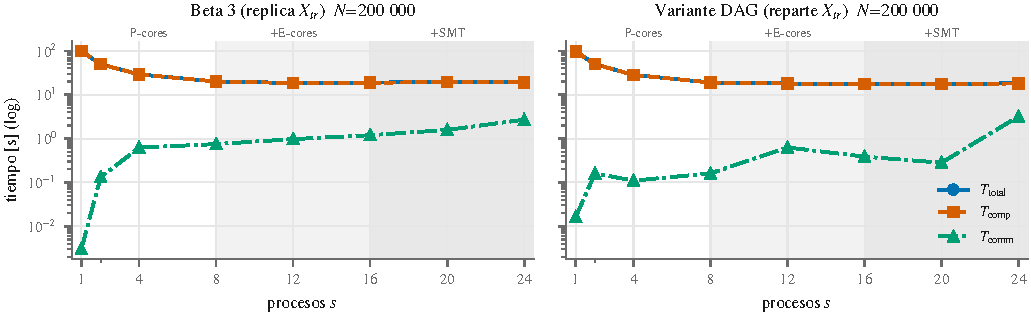
\includegraphics[width=0.92\linewidth, height=0.50\textheight, keepaspectratio]{f2_tiempos.pdf}
\pieFig{$N=200\,000$ ($\ntr=160\,000$, $\mte=40\,000$). Bandas: P-cores ($s\le8$), +E-cores, +SMT ($s>16$).}
\vspace{0.15cm}

\begin{columns}[T,onlytextwidth]
    \begin{column}{0.25\textwidth}
        \kpi{98.5\,s $\to$ 18.6\,s}{$T_{\text{total}}$ con $s=1$ y $s=12$}
    \end{column}
    \begin{column}{0.17\textwidth}
        \kpi{$>$99\,\%}{del tiempo es cómputo}
    \end{column}
    \begin{column}{0.52\textwidth}
        \cajaAlert{\linewidth}{%
            \encCaja{Observación clave}
            Desde $s=8$, $\Tcomp$ \textbf{deja de bajar}: cada proceso hace $W/s$ operaciones pero
            tarda lo mismo. El crecimiento de $\Tcomm$ para $s\ge16$ es espera por desbalance.
        }
    \end{column}
\end{columns}
\end{frame}

% ------------------------------------------------------------------------------
\begin{frame}{Speedup y Ley de Amdahl (escalabilidad fuerte)}
\footnotesize
\centering
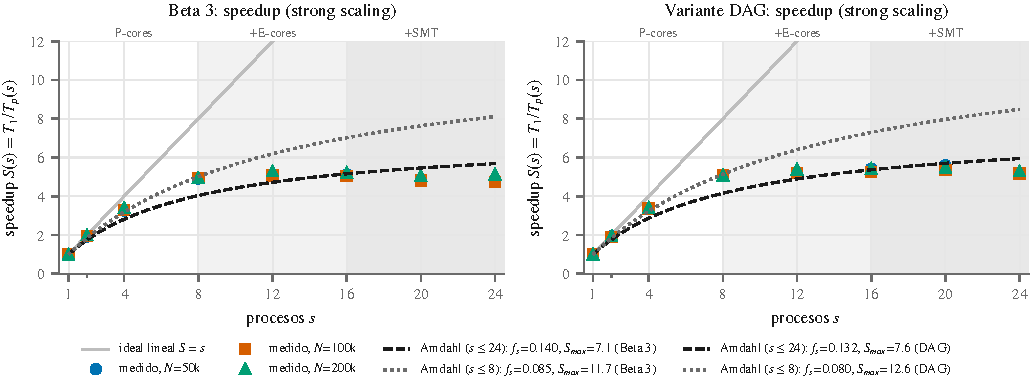
\includegraphics[width=0.92\linewidth, height=0.53\textheight, keepaspectratio]{f3_speedup.pdf}
\vspace{0.1cm}

\begin{columns}[T,onlytextwidth]
    \begin{column}{0.15\textwidth}
        \kpi{5.29}{$S$ máximo medido ($s=12$)}
    \end{column}
    \begin{column}{0.24\textwidth}
        \cajaInfo{\linewidth}{%
            \encCaja{Ley de Amdahl}
            \centering$S(s)=\dfrac{1}{f_s+f_p/s}$\\[0.1cm]
            $S_{\max}=1/f_s$
        }
    \end{column}
    \begin{column}{0.19\textwidth}
        \centering
        \renewcommand{\arraystretch}{1.1}
        \begin{tabular}{@{}lcc@{}}
            \toprule
            Ajuste & $f_s$ & $S_{\max}$\\
            \midrule
            $s\le 24$ & 0.140 & 7.1\\
            $s\le 8$ & 0.085 & 11.7\\
            \bottomrule
        \end{tabular}
    \end{column}
    \begin{column}{0.36\textwidth}
        \cajaAlert{\linewidth}{%
            $f_s\approx0.14$ \textbf{no es código serial} (éste es menor al 1\,\%): es una fracción
            serial \emph{efectiva} por \textbf{contención del bus DDR5}. Los tres $N$ dan la misma curva.
        }
    \end{column}
\end{columns}
\end{frame}

% ------------------------------------------------------------------------------
\begin{frame}{Normalización del modelo teórico y proceso óptimo $s^*$}
\footnotesize
\begin{columns}[T,onlytextwidth]
    \begin{column}{0.40\textwidth}
        \cajaInfo{\linewidth}{%
            \encCaja{Modelo normalizado}
            $$T_p(s)=k_1\,\frac{W}{s}+k_2\,\Tcomm(s)$$
            {\scriptsize $W=3\,\mte\ntr d$. Lineal: $\Tcomm=(s-1)(\alpha+M\beta)$;\\
            árbol: $\Tcomm=\log_2 s\,(\alpha+M\beta)$.}
        }
        \vspace{0.1cm}

        \cajaAcento{\linewidth}{%
            \encCaja{Procedimiento}
            1.\ $\alpha,\beta$ medidos con colectivas aisladas.\\
            2.\ $k_1,k_2$ por mínimos cuadrados sobre $T$ medido.\\
            3.\ $\dfrac{dT_p}{ds}=-\dfrac{k_1W}{s^2}+k_2c=0$
            $$\Rightarrow\ \boxed{s^*=\sqrt{\dfrac{k_1W}{k_2\,c}}}$$
        }
    \end{column}
    \begin{column}{0.57\textwidth}
        \centering
        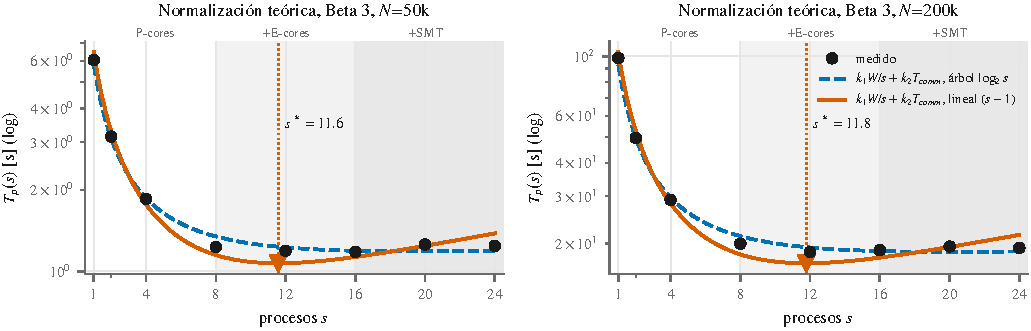
\includegraphics[width=\linewidth]{f6_modelo.pdf}
        \vspace{0.05cm}

        \renewcommand{\arraystretch}{1.1}
        \begin{tabular}{@{}lcccc@{}}
            \toprule
            Modelo ($N$=200k) & $k_1$ [s/FLOP] & $k_2$ & error & $s^*$\\
            \midrule
            Árbol & $7.6\times10^{-11}$ & 139 & 3.4\,\% & 19.9\\
            \textbf{Lineal} & $8.4\times10^{-11}$ & 122 & 6.4\,\% & \textbf{11.8}\\
            \midrule
            \multicolumn{4}{@{}l}{\textbf{Mínimo experimental}} & \textbf{12}\\
            \bottomrule
        \end{tabular}
        \vspace{0.12cm}

        \kpi{$s^*_{\text{teórico}}=11.8$ \quad vs. \quad $s^*_{\text{medido}}=12$}{modelo de comunicación lineal, $N=200$k}
    \end{column}
\end{columns}
\end{frame}

% ------------------------------------------------------------------------------
\begin{frame}{Interpretación de la normalización}
\footnotesize
\begin{columns}[T,onlytextwidth]
    \begin{column}{0.31\textwidth}
        \cajaInfo{\linewidth}{%
            \encCaja{$1/k_1\approx 12$ GFLOP/s}
            Es el rendimiento medido de \textbf{un P-core aislado}. Estable entre los tres tamaños de
            problema.
        }
    \end{column}
    \begin{column}{0.31\textwidth}
        \cajaAlert{\linewidth}{%
            \encCaja{$k_2\gg 1$ y crece con $N$}
            Si sólo costaran los mensajes, $k_2\approx 1$. El exceso es la \textbf{competencia por el
            bus de memoria}: cada proceso recorre $\Xtr$ (80\,MB $>$ 30\,MB de L3). Cuello de botella de
            \textbf{von Neumann}.
        }
    \end{column}
    \begin{column}{0.31\textwidth}
        \cajaOk{\linewidth}{%
            \encCaja{$s^*$ no depende de $N$}
            $W\propto N^2$ y $k_2c\propto N\cdot N$ $\Rightarrow$ $s^*\approx$ 11.4--11.8 para
            50k, 100k y 200k, igual al mínimo medido ($s=12$).
        }
    \end{column}
\end{columns}
\vspace{0.4cm}

\begin{center}
\cajaAcento{0.82\textwidth}{%
    \centering
    {\normalsize\bfseries Cantidad óptima de procesos: $s^*\approx 12$} \quad (8 P-cores + 4 E-cores)\\[0.1cm]
    {\scriptsize Entre $s=12$ y $s=24$ el tiempo varía menos del 5\,\%: mismo resultado con la mitad de los recursos.}
}
\end{center}
\end{frame}

% ------------------------------------------------------------------------------
\begin{frame}{Rendimiento en FLOP/s y eficiencia}
\footnotesize
\begin{columns}[T,onlytextwidth]
    \begin{column}{0.40\textwidth}
        \centering
        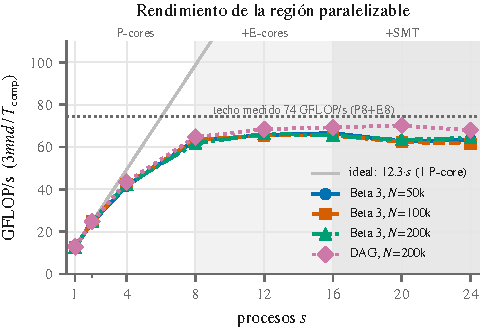
\includegraphics[width=\linewidth]{f5_gflops.pdf}
        \pieFig{$\text{GFLOP/s}=3\,\mte\ntr d\,/\,(\Tcomp\cdot10^9)$.}
    \end{column}
    \begin{column}{0.40\textwidth}
        \centering
        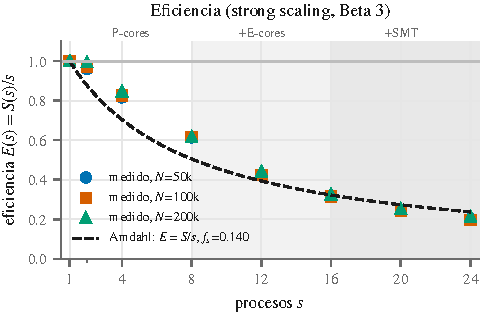
\includegraphics[width=\linewidth]{f4_eficiencia.pdf}
        \pieFig{$E(s)=S(s)/s$ medida y predicha por Amdahl.}
    \end{column}
    \begin{column}{0.17\textwidth}
        \kpi{12.5}{GFLOP/s con $s=1$}\\[0.12cm]
        \kpi{66 / 70}{GFLOP/s Beta 3 / DAG}\\[0.12cm]
        \kpi{74.3}{GFLOP/s techo medido}\\[0.12cm]
        \kpi{0.21}{eficiencia $E(24)$}
    \end{column}
\end{columns}
\vspace{0.1cm}
\cajaInfo{\textwidth}{%
    Con $\ntr$ fijo $E(s)\to0$: el algoritmo \textbf{no es fuertemente escalable} en esta máquina. El
    rendimiento depende de los núcleos activos y de su acceso compartido a memoria, \textbf{no de $N$}.
}
\end{frame}

% ------------------------------------------------------------------------------
\begin{frame}{Escalabilidad débil y Ley de Gustafson}
\footnotesize
\centering
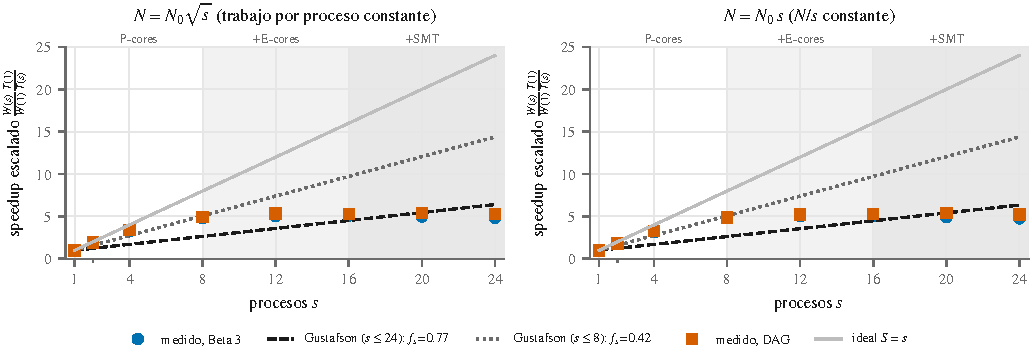
\includegraphics[width=0.92\linewidth, height=0.52\textheight, keepaspectratio]{f7_debil.pdf}
\vspace{0.1cm}

\begin{columns}[T,onlytextwidth]
    \begin{column}{0.24\textwidth}
        \cajaInfo{\linewidth}{%
            \encCaja{Ley de Gustafson}
            $S(s)=f_s+s\,f_p$
        }\\[0.1cm]
        \kpi{0.20}{$E_{\text{débil}}(24)$}
    \end{column}
    \begin{column}{0.36\textwidth}
        \cajaAlert{\linewidth}{%
            \encCaja{Detalle clave: $W\propto N^2$}
            $N/s$ constante \textbf{no} fija el trabajo por proceso ($W/s\propto s$).
            Lo correcto es $N=N_0\sqrt{s}$.
        }
    \end{column}
    \begin{column}{0.36\textwidth}
        \cajaAcento{\linewidth}{%
            Con trabajo constante: 5.9 $\to$ 29.4\,s ($E=0.20$ con $s=24$), $f_s=0.42$ ($s\le8$).
            Aumentar $N$ \textbf{no añade canales de memoria}.
        }
    \end{column}
\end{columns}
\end{frame}

% ==============================================================================
\seccion{4}{\textquestiondown{}Por qué se satura?}{Comunicación lineal vs.\ árbol, núcleos P/E y SMT}
% ==============================================================================

% ------------------------------------------------------------------------------
\begin{frame}{Modelo de comunicación: lineal vs.\ árbol binario}
\footnotesize
\centering
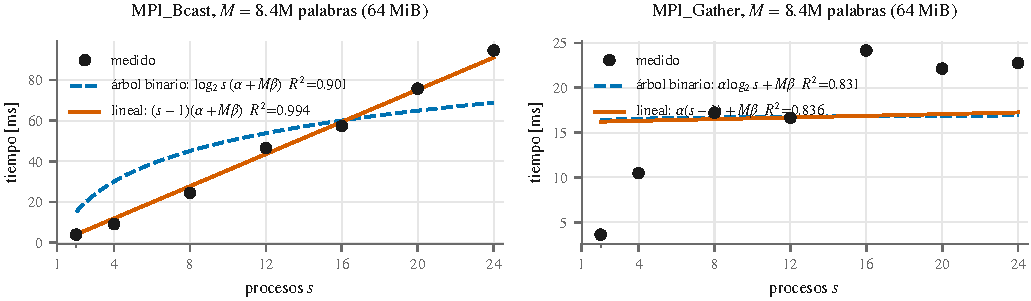
\includegraphics[width=0.90\linewidth, height=0.50\textheight, keepaspectratio]{f9_comunicacion.pdf}
\pieFig{Colectivas sin cómputo, mensaje de 64\,MiB. Ajuste con 9 tamaños de mensaje y 7 valores de $s$.}
\vspace{0.1cm}

\begin{columns}[T,onlytextwidth]
    \begin{column}{0.32\textwidth}
        \centering
        \renewcommand{\arraystretch}{1.1}
        \begin{tabular}{@{}lcc@{}}
            \toprule
            \texttt{Bcast} & Modelo (Unidad 2) & $R^2$\\
            \midrule
            Árbol & $O(\log p\,(\alpha+m\beta))$ & 0.901\\
            \textbf{Lineal} & $O(p\,(\alpha+m\beta))$ & \textbf{0.994}\\
            \bottomrule
        \end{tabular}
    \end{column}
    \begin{column}{0.30\textwidth}
        \cajaAlert{\linewidth}{%
            De $s=2$ a $s=24$ el \texttt{Bcast} crece \textbf{24$\times$} (3.9 $\to$ 94.5\,ms):
            es $O(s)$, no $O(\log s)$.
        }
    \end{column}
    \begin{column}{0.34\textwidth}
        \cajaInfo{\linewidth}{%
            Sin enlaces independientes, las $s-1$ copias \textbf{compiten por el bus DDR5}. En el
            KNN el \texttt{Bcast} es menos del 1\,\% del tiempo.
        }
    \end{column}
\end{columns}
\end{frame}

% ------------------------------------------------------------------------------
\begin{frame}{Justificación de hardware: núcleos P, núcleos E y SMT}
\footnotesize
\begin{columns}[T,onlytextwidth]
    \begin{column}{0.60\textwidth}
        \centering
        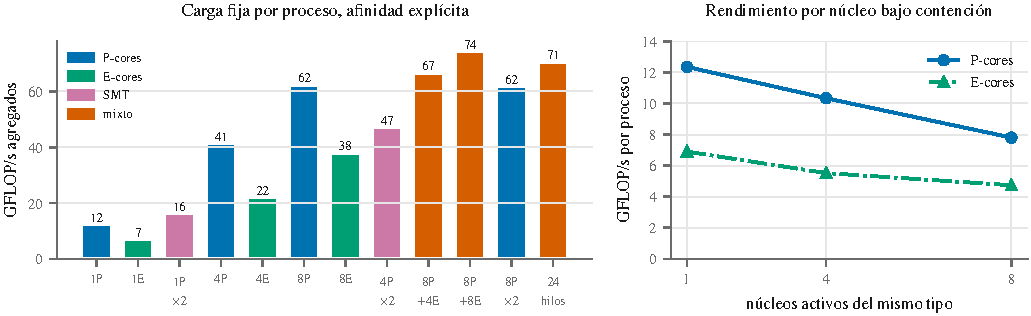
\includegraphics[width=\linewidth]{f8_pinning.pdf}
        \pieFig{Misma carga por proceso, cada proceso fijado a una CPU lógica concreta.}
        \vspace{0.15cm}

        \cajaAcento{\linewidth}{\scriptsize\itshape
            ``No se recomienda usar todos los hilos de un CPU [\ldots] Pasado cierto punto, cada hilo
            extra aporta poco o incluso resta. Debido a: Ancho de banda de memoria, [\ldots] SMT no
            equivale a núcleos reales, [\ldots] Desbalance de carga. El óptimo suele estar en un punto
            intermedio.''\ \upshape --- Fiestas, Unidad 4, pág.~22
        }
    \end{column}
    \begin{column}{0.37\textwidth}
        \cajaInfo{\linewidth}{%
            \encCaja{1. Ancho de banda DRAM saturado}
            P-core: 12.3 GFLOP/s solo $\to$ 10.3 (4 activos) $\to$ 7.8 (8 activos).
        }\\[0.12cm]
        \cajaInfo{\linewidth}{%
            \encCaja{2. SMT no es núcleo real (+30\,\%)}
            2 hilos en 1 P-core: +30\,\%. 8 P físicos: 62 vs.\ 4P$\times$2: 47 GFLOP/s.
        }\\[0.12cm]
        \cajaInfo{\linewidth}{%
            \encCaja{3. Desbalance P-core vs.\ E-core}
            E-core = mitad de un P-core (6.9 vs.\ 12.3). Los rápidos esperan en \texttt{Gatherv}.
        }\\[0.12cm]
        \cajaOk{\linewidth}{%
            $s^*=12$ es el ``punto intermedio'' de la diapositiva del curso.
        }
    \end{column}
\end{columns}
\end{frame}

% ------------------------------------------------------------------------------
\begin{frame}{Beta 3 vs.\ variante DAG y mejoras propuestas}
\footnotesize
\begin{columns}[T,onlytextwidth]
    \begin{column}{0.48\textwidth}
        \renewcommand{\arraystretch}{1.15}
        \begin{tabular}{@{}rrrr@{}}
            \toprule
            $s$ & Beta 3 [s] & DAG [s] & Fusión DAG [s]\\
            \midrule
            1  & 98.46 & 96.52 & 0.006\\
            8  & 19.97 & 19.03 & 0.018\\
            12 & 18.60 & 18.01 & 0.025\\
            16 & 18.90 & 17.82 & 0.043\\
            24 & 19.26 & 18.23 & 0.056\\
            \bottomrule
        \end{tabular}
        \pieFig{$N=200\,000$. Ambas producen predicciones idénticas.}
        \vspace{0.15cm}

        \cajaOk{\linewidth}{%
            \encCaja{DAG: 2--6\,\% más rápida}
            Evita el \texttt{Bcast} de $\Xtr$ y cada proceso recorre sólo $\ntr/s$ puntos
            $\Rightarrow$ \textbf{menos tráfico a memoria}. La fusión serial es despreciable con $k=3$.
        }
    \end{column}
    \begin{column}{0.48\textwidth}
        \cajaInfo{\linewidth}{%
            \encCaja{Mejoras propuestas}
            \begin{itemize}
                \setlength{\itemsep}{0.3em}
                \item \textbf{Reparto ponderado} en \texttt{Scatterv}: P-core $\approx 2\times$ E-core.
                \item \textbf{Afinidad explícita} a P-cores físicos con $s\le8$.
                \item \textbf{Bloqueo por caché}: reutilizar bloques de $\Xtr$ en L2 para varias
                      consultas.
                \item \textbf{Memoria distribuida} (clúster): cada nodo aporta su canal de memoria;
                      ahí aplica el modelo en árbol y Gustafson.
            \end{itemize}
        }
    \end{column}
\end{columns}
\end{frame}

% ------------------------------------------------------------------------------
\begin{frame}{Conclusiones}
\footnotesize
\vspace{0.1cm}
\begin{columns}[T,onlytextwidth]
    \begin{column}{0.48\textwidth}
        \cajaInfo{\linewidth}{%
            \encCaja{1. Diseño correcto}
            PCAM + PRAM CREW con \texttt{forall \ldots\ pardo}. Tres betas y DAG validadas al
            100\,\% contra el secuencial y scikit-learn.
        }\\[0.15cm]
        \cajaInfo{\linewidth}{%
            \encCaja{2. Desarrollo incremental}
            Vectorización $\sim$156$\times$, buffers +33\,\%; hasta $\sim$1000$\times$ frente al
            código original con 8 procesos.
        }\\[0.15cm]
        \cajaOk{\linewidth}{%
            \encCaja{3. Teoría vs.\ experimento}
            $T_p=k_1W/s+k_2\Tcomm$ (modelo lineal): error 6\,\% y $s^*=11.8$ vs.\ 12 medido.
        }
    \end{column}
    \begin{column}{0.48\textwidth}
        \cajaAlert{\linewidth}{%
            \encCaja{4. Límite de escalabilidad}
            $S_{\max}\approx 5.3$ ($f_s=0.14$), $E(24)=0.21$; Gustafson tampoco se cumple. La causa
            demostrada: bus de memoria, SMT y desbalance P/E, \textbf{no MPI}.
        }\\[0.15cm]
        \cajaInfo{\linewidth}{%
            \encCaja{5. Comunicación en memoria compartida}
            Las colectivas siguen el modelo \textbf{lineal} $O(s)$ ($R^2=0.994$): cuello de botella de
            von Neumann.
        }\\[0.15cm]
        \cajaAcento{\linewidth}{%
            \encCaja{Recomendación}
            Usar $s\approx 12$ procesos, no los 24 hilos disponibles.
        }
    \end{column}
\end{columns}
\end{frame}

% ------------------------------------------------------------------------------
\begin{frame}{Fuentes y Bibliografía Destacada}
\footnotesize
\vspace{0.2cm}
\begin{columns}[T,onlytextwidth]
    \begin{column}{0.48\textwidth}
        \cajaInfo{\linewidth}{%
            \encCaja{Base teórica}
            J.~Fiestas, \emph{Unidades 1--4: Modelos PRAM, MPI, Leyes de Escalabilidad y
            Arquitecturas Híbridas}, CS4052, UTEC, 2026.
        }\\[0.2cm]
        \cajaInfo{\linewidth}{%
            \encCaja{Desarrollo MPI}
            L.~Dalcín, \emph{MPI for Python (mpi4py) documentation}, 2025.
        }
    \end{column}
    \begin{column}{0.48\textwidth}
        \cajaAcento{\linewidth}{%
            \encCaja{Leyes de escalabilidad}
            G.~M.~Amdahl (1967), \emph{Validity of the Single Processor Approach\ldots}\\
            J.~L.~Gustafson (1988), \emph{Reevaluating Amdahl's Law}.
        }\\[0.2cm]
        \cajaAcento{\linewidth}{%
            \encCaja{Especificaciones de hardware}
            Intel Corp., \emph{Intel Core i7-14650HX Processor Specifications}, 2024.
        }
    \end{column}
\end{columns}
\vspace{0.3cm}
\begin{center}
{\scriptsize\color{UTECGray}Bibliografía completa (36 referencias) en la Sec.~5 del informe final.}
\end{center}
\end{frame}

% ------------------------------------------------------------------------------
% CIERRE
% ------------------------------------------------------------------------------
\begin{frame}[plain]
    \begin{tikzpicture}[remember picture,overlay]
        \fill[UTECCyan] (current page.south west) rectangle ([xshift=0.4cm]current page.north west);
    \end{tikzpicture}

    \vfill
    \begin{center}
        {\Large\color{UTECDarkBlue}\bfseries \textexclamdown{}Muchas gracias por su atención!}

        \vspace{0.3cm}
        \tikz\draw[UTECCyan, line width=2pt] (0,0) -- (4.2,0);

        \vspace{0.6cm}
        {\small\color{UTECDarkBlue}\bfseries Paralelización del clasificador KNN con MPI} \\[0.25cm]

        {\footnotesize\color{UTECGray}
        Juan David Velo Poma \quad $\cdot$ \quad Farid Jack Aquino Castro \quad $\cdot$ \quad Josue Nehemias Velo Poma}

        \vspace{0.5cm}
        {\scriptsize\color{UTECGray}Universidad de Ingeniería y Tecnología (UTEC) -- 2026}
    \end{center}
    \vfill
\end{frame}

% ==============================================================================
% ANEXO (diapositivas de respaldo para preguntas)
% ==============================================================================
\appendix
\seccion{A}{Anexo}{Diapositivas de respaldo para la ronda de preguntas}

% ------------------------------------------------------------------------------
\begin{frame}[fragile]{Anexo: Algoritmo Beta 1 (Comunicación básica)}
\begin{columns}[T,onlytextwidth]
    \begin{column}{0.67\textwidth}
\begin{lstlisting}
# Rango 0: carga, divide y prepara bloques (m % s != 0 admitido)
if rank == 0:
    X_train, X_test, y_train, y_test = train_test_split(
        X, y, test_size=0.2, random_state=42)
    test_chunks = np.array_split(X_test, size)

X_train = comm.bcast(X_train, root=0)    # pickle: replica X_tr
y_train = comm.bcast(y_train, root=0)
X_local = comm.scatter(test_chunks, root=0)  # bloque de consultas

# Cómputo local IDÉNTICO al secuencial: bucle Python por punto
def knn_predict(test_point, X_train, y_train, k):
    distances = [euclidean_distance(test_point, x) for x in X_train]
    k_indices = np.argsort(distances)[:k]
    k_labels = [y_train[i] for i in k_indices]
    return Counter(k_labels).most_common(1)[0][0]

y_local = [knn_predict(x, X_train, y_train, k) for x in X_local]
gathered = comm.gather(y_local, root=0)  # pickle: recolección
\end{lstlisting}
    \end{column}
    \begin{column}{0.30\textwidth}
        \footnotesize
        \cajaInfo{\linewidth}{%
            \encCaja{Idea}
            Paralelizar \textbf{sin tocar el cómputo}: sólo cambia la descomposición de datos.
        }\\[0.15cm]
        \cajaAcento{\linewidth}{%
            \encCaja{Colectivas genéricas}
            \texttt{bcast}, \texttt{scatter}, \texttt{gather} en minúscula serializan objetos
            con \emph{pickle}.
        }\\[0.15cm]
        \cajaOk{\linewidth}{%
            \encCaja{Resultado}
            Exactitud 0.9833; $S(8)=6.7$ ($E=0.83$) sobre el secuencial.
        }
    \end{column}
\end{columns}
\end{frame}

% ------------------------------------------------------------------------------
\begin{frame}[fragile]{Anexo: Algoritmo Beta 2 (Vectorización local)}
\begin{columns}[T,onlytextwidth]
    \begin{column}{0.67\textwidth}
\begin{lstlisting}
def knn_predict_block(X_train, y_train, sq_train, Q, k):
    # ||q - x||^2 = ||q||^2 + ||x||^2 - 2 q.x   (b x n, sin bucles)
    D2 = np.einsum("ij,ij->i", Q, Q)[:, None] + sq_train[None, :] \
         - 2.0 * (Q @ X_train.T)              # producto matricial (BLAS)
    D = np.sqrt(np.maximum(D2, 0.0))          # distancia euclidiana
    nn = np.argpartition(D, k - 1, axis=1)[:, :k]   # k vecinos en O(n)
    votes = np.zeros((Q.shape[0], 10), dtype=np.int64)
    np.add.at(votes, (np.arange(Q.shape[0])[:, None], y_train[nn]), 1)
    return votes.argmax(axis=1)               # moda vectorizada

t0 = MPI.Wtime()
X_train = comm.bcast(X_train, root=0)         # comunicación aún pickle
t1 = MPI.Wtime()
X_local = comm.scatter(test_chunks, root=0)
t2 = MPI.Wtime()
y_local = knn_local(X_train, y_train, X_local, k, block=256)
t3 = MPI.Wtime()                              # T_comp = t3 - t2
gathered = comm.gather(y_local, root=0)
\end{lstlisting}
    \end{column}
    \begin{column}{0.30\textwidth}
        \footnotesize
        \cajaInfo{\linewidth}{%
            \encCaja{Cambio clave}
            El bucle Python de $\ntr$ iteraciones se reemplaza por \texttt{np.einsum} y un producto
            matricial por bloques de 256 consultas.
        }\\[0.15cm]
        \cajaAcento{\linewidth}{%
            \encCaja{Instrumentación}
            \texttt{MPI.Wtime()} por fase: $\Tcomp$ y $\Tcomm$ separados (máximo entre procesos).
        }\\[0.15cm]
        \cajaOk{\linewidth}{%
            \encCaja{Resultado}
            $\sim$156$\times$ más rápida que la Beta 1 con $s=1$; misma exactitud (0.9833).
        }
    \end{column}
\end{columns}
\end{frame}

% ------------------------------------------------------------------------------
\begin{frame}{Respaldo: derivación de $s^*$ en ambos modelos}
\footnotesize
\begin{columns}[T,onlytextwidth]
    \begin{column}{0.48\textwidth}
        \cajaInfo{\linewidth}{%
            \encCaja{Modelo lineal}
            $$T_p(s)=k_1\frac{W}{s}+k_2\,c\,(s-1),\quad c=\alpha+M\beta$$
            $$\frac{dT_p}{ds}=-\frac{k_1W}{s^2}+k_2c=0\ \Rightarrow\ s^*=\sqrt{\frac{k_1W}{k_2c}}$$
            $N$=200k: $k_1W=103.8$\,s, $k_2c=0.748$\,s $\Rightarrow$ $s^*=11.8$.
        }
    \end{column}
    \begin{column}{0.48\textwidth}
        \cajaAcento{\linewidth}{%
            \encCaja{Modelo en árbol}
            $$T_p(s)=k_1\frac{W}{s}+k_2\,c\log_2 s$$
            $$-\frac{k_1W}{s^2}+\frac{k_2c}{s\ln2}=0\ \Rightarrow\ s^*=\frac{k_1W\ln2}{k_2c}$$
            Predice $s^*\approx 20$ (zona SMT): no reproduce el aumento de $T_p$ tras el mínimo.
        }
    \end{column}
\end{columns}
\vspace{0.25cm}
\cajaInfo{\textwidth}{%
    $M=\ntr(d+1)+\mte d+\mte$ palabras (\texttt{Bcast} de $\Xtr,y_{\text{tr}}$ + \texttt{Scatterv} de $\Xte$ +
    \texttt{Gatherv} de $\hat y$). $W=3\,\mte\ntr d = 1.23\times10^{12}$ FLOPs con $N=200$k.
}
\end{frame}

% ------------------------------------------------------------------------------
\begin{frame}{Respaldo: escalabilidad fuerte completa ($N=200\,000$, Beta 3)}
\footnotesize
\centering
\renewcommand{\arraystretch}{1.15}
\begin{tabular}{rrrrrrr}
    \toprule
    $s$ & $T_{\text{total}}$ [s] & $\Tcomp$ [s] & $\Tcomm$ [s] & $S(s)$ & $E(s)$ & GFLOP/s\\
    \midrule
    1 & 98.46 & 98.46 & 0.003 & 1.00 & 1.00 & 12.5\\
    2 & 49.53 & 49.51 & 0.131 & 1.99 & 0.99 & 24.8\\
    4 & 29.09 & 29.06 & 0.623 & 3.39 & 0.85 & 42.3\\
    8 & 19.97 & 19.93 & 0.749 & 4.93 & 0.62 & 61.7\\
    12 & 18.60 & 18.54 & 0.972 & \textbf{5.29} & 0.44 & 66.3\\
    16 & 18.90 & 18.80 & 1.195 & 5.21 & 0.33 & 65.4\\
    20 & 19.50 & 19.39 & 1.574 & 5.05 & 0.25 & 63.4\\
    24 & 19.26 & 19.11 & 2.705 & 5.11 & 0.21 & 64.3\\
    \bottomrule
\end{tabular}

\vspace{0.3cm}
\cajaInfo{0.85\textwidth}{%
    $\Tcomm$ incluye la espera en las colectivas por el proceso más lento (desbalance). El
    \texttt{Bcast} puro de $\Xtr$ (83\,MB) cuesta 0.15\,s con $s=24$: 0.8\,\% del total.
}
\end{frame}

\end{document}
